\section{Introduction}
\label{sec:intro}

Brain--computer interfaces (BCIs) for text entry are moving towards clinical and consumer use. Intracortical neuroprostheses decode attempted speech, handwriting and typing at high rates \citep{willett2023speech,card2024accurate,metzger2023avatar,willett2021handwriting,jude2026bimanual}; non-invasive decoders reconstruct typed sentences from magnetoencephalography (MEG) \citep{levy2026brain2qwerty,zhang2026brain2qwertyv2}; and surface electromyography (sEMG) is a candidate input for wearables \citep{sivakumar2024emg2qwerty,achituve2025emg,ctrllabs2025generic}. Most of these systems end in a language-model (LM) stage that turns noisy per-frame predictions into sentences. This lowers the error rate but changes the kind of error: when the neural evidence is weak, the LM still returns a grammatical sentence, and a reader has no cue that it is wrong. In speech recognition, such fluent unsupported output has caused documented harm \citep{koenecke2024careless}.

For people who depend on the interface to communicate, accuracy is a stated priority \citep{huggins2011als,huggins2015sci,blabe2015assessment,kubler2014ucd}, and users of augmentative and alternative communication (AAC) want LM-generated text to reflect their own intent \citep{valencia2023aac,kane2017avuncular}. A sentence sent in their name that they did not mean is a harm in itself. Current speech neuroprostheses read a finalised sentence aloud without a confirmation step \citep{card2024accurate} or synthesise voice instantaneously \citep{wairagkar2025voice}. Whether a decoded sentence should be sent without confirmation (\emph{committed}) is therefore a real design decision.

Sentence-level LM decoders for speech, handwriting, typing and sEMG share one structure: per-frame probabilities followed by an LM search. A commit rule can therefore act on the per-frame output instead of inside one decoder. The statistical tools exist: calibration, selective classification, conformal risk control (CRC) and Learn-then-Test (LTT) \citep{guo2017calibration,geifman2017selective,bates2021rcps,angelopoulos2024crc,angelopoulos2025ltt}. They have been applied to single BCI decoders \citep{kim2025confidence,huang2025cocontrol} and to speech recognition \citep{damri2026risk}. The methods are not new. What is missing is their use as a commit rule for neural text entry, a test of the guarantee when calibration comes before use in time, and the fair comparators: ``always offer, never commit'' and a no-BCI baseline such as gaze typing \citep{cai2024gaze}.

\paragraph{This work.} We define the problem (\cref{sec:setting}), a trust layer on a per-frame output stream (\cref{sec:trust}) and an evaluation protocol (\cref{sec:protocol}), and test them offline on public data. Our contributions are:
\begin{enumerate}[leftmargin=*,itemsep=1pt]
  \item \textbf{A stream-level commit rule with a stated guarantee.} The layer calibrates the per-frame log-probabilities and chooses \act{commit}, \act{offer} or \act{abstain}. LTT with a max rule bounds the wrong-commit rate with high probability (Algorithm~\ref{alg:decide}; Algorithm~\ref{alg:calibrate} in the supplement).
  \item \textbf{A time-ordered test of the guarantee on one participant.} We calibrate on earlier days or on the start of a session and test on later data, over 14 days. We also show the scope of the guarantee: it bounds the risk over the mix of days, not on each day.
  \item \textbf{A safety-first evaluation protocol}: the wrong-commit rate with the commit rate and the error among commits; always-commit, always-offer and gaze-typing baselines; a simulated-user speed metric with a sensitivity analysis; and signal-destroying controls. These controls show that a plain confidence threshold commits no-information streams, so a commit rule needs an input-validity check.
\end{enumerate}
The stream format (\nts{} v0.1), its adapters, an audit log and all scripts are released under Apache-2.0. The sEMG and MEG data show that one format and one code path work across devices; they do not show that the commit rule works across decoders.

\Cref{fig:teaser} summarises the result. On the one intracortical participant, the layer turned frequent wrong commits into rare ones. On composed sEMG sentences it committed few sentences, and on MEG it never committed. Its speed gains over the same policy without commits were small (about 1\% and 3\%) and depend on the user model, and on the published decoder always committing was faster, so our claim is about safety.

\begin{figure}[t]
  \centering
  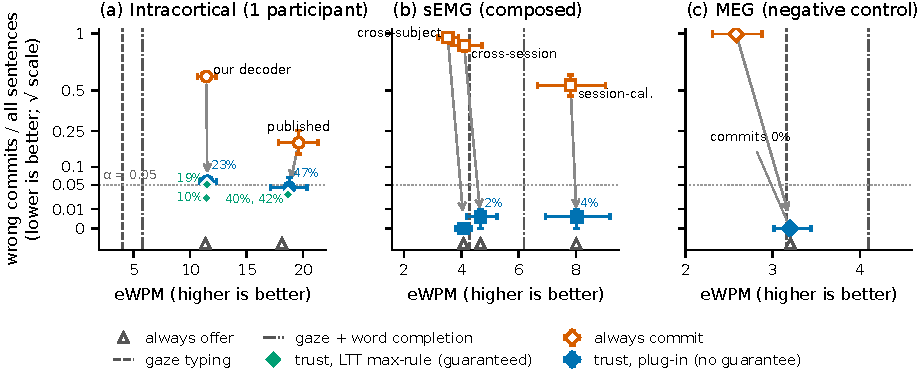
\includegraphics[width=\linewidth]{fig1_teaser.pdf}
  \caption{\textbf{The trust layer turns frequent wrong commits into rare ones; on MEG it does so by never committing.} Wrong commits per sentence attempted (signed square-root axis) against effective words per minute (\ewpm{}) of a simulated user. Open markers: always commit; blue: plug-in trust layer (full fit, no guarantee); green diamonds: the guaranteed rule (fit-A pipeline, guard, clean calibration, LTT max rule; fixed splits A and B); triangles: always offer (no wrong commits; drawn just below 0). Labels give the commit rate. Dashed line: gaze typing; dash-dotted: gaze typing with word completion; dotted: $\alpha = 0.05$. Error bars: 95\% cluster-bootstrap CIs over days (a), participants (b) and sentences $\times$ participants (c), conditional on the fitted pipeline. (a)~Intracortical speech, one participant, 816 test trials. (b)~sEMG, 551 composed sentences, 19 participants; the guaranteed rule gives the same rates as the plug-in rule (not drawn). (c)~MEG typing, 637 instances of 17 sentences; the layer equals always offer.}
  \label{fig:teaser}
\end{figure}
